
\documentclass[10pt]{article}

\def\Type{LessonDJ}
\def\TypeNum{Lesson 26}
\def\TypeTitle{Final Exam Review}
\def\Semester{Fall 2021} %Not Used 
\def\Course{MATH 1190 \& 1210}
\def\Targets{  }

\usepackage{preambleDJ}

%\usepackage{ragged2e}


%%%%%%%%%%%% BEGIN DOCUMENT %%%%%%%%%%%%%%%
%%%%%%%%%%%% BEGIN DOCUMENT %%%%%%%%%%%%%%%
%%%%%%%%%%%% BEGIN DOCUMENT %%%%%%%%%%%%%%%
%%%%%%%%%%%% BEGIN DOCUMENT %%%%%%%%%%%%%%%
%%%%%%%%%%%% BEGIN DOCUMENT %%%%%%%%%%%%%%%

%\usepackage{array}   % for \newcolumntype macro
%\newcolumntype{L}{>{$}l<{$}} % math-mode version of "l" column type
%\newcolumntype{C}{>{$}c<{$}} % math-mode version of "l" column type

\newcommand{\rowstyle}[1]{\gdef\currentrowstyle{#1}}

\usepackage{diagbox}

\def\sz{.2}

\begin{document}

\pagestyle{otherpages}
\thispagestyle{firstpage}
\vs{.25}
\section{Limits with Continuity and Forms}
\def\szz{1.15}
\enum{
\item \ltrm{\target{L2}}Evaluate the following limits using continuity or a specific form.  If you use continuity to evaluate a limit, to receive full credit, please provide sufficient explanation for why continuity can be used, including why the given function is continuous at the given point.
\enum{
\mpageTTh{.2}{.2}{.6}{
\item $\ds \limx \frac{x^3+e^x-2}{x^3+x^5}$
}{
Form:  \blue{
$\ds \frac{\infty}{\infty}$
}
}{
Value: 
\begin{solution}
Since $x\to\infty$ we examine fastest growing terms in numerator and denominator.
$$\ds \limx \frac{x^3+e^x-2}{x^3+x^5}\sim  \limx \frac{e^x}{x^5}$$
The exponential function $e^x$ grows faster than the polynomial $x^5$ so $\ds  \limx \frac{e^x}{x^5}=\infty$ and thus 
$$\ds \limx \frac{x^3+e^x-2}{x^3+x^5}=\infty.$$
\end{solution}
}
~\\
\mpageTTh{.2}{.2}{.6}{
\item $\ds \lim_{x\to 0^-} \frac{x^3+e^x-2}{x^3+x^5}$
}{
Form:
\blue{
$\ds \frac{c}{0}$
}
}{
Value:
\begin{solution}
$\ds \lim_{x\to 0^-} \frac{x^3+e^x-2}{x^3+x^5} =\frac{0+e^0-2}{0^3+0^5}=\frac{-1}{0}$ which tells us that the form is $\ds \frac{c}{0}$. \\\\
We now need to determine how the denominator approaches $0$. Since $x\to 0^-$ $x$ is getting lose to $0$ from the left, i.e. with negative values. \\\\
For example when $x=-0.1$, the denominator is $(-0.1)^3+(-0.1)^5=-0.001-0.00001$ which is negative. Thus
$$\ds \lim_{x\to 0^-} \frac{x^3+e^x-2}{x^3+x^5}\to \frac{-1}{0^-}=+\infty$$
\end{solution}
}
~\\
\mpageTTh{.2}{.2}{.6}{
\item $\ds \lim_{x\to 2^+} \frac{x^3+e^x-2}{x^3+x^5}$
}{
Form: \blue{ N/A}
}{
Value:
\begin{solution}
$\ds \lim_{x\to 2^+} \frac{x^3+e^x-2}{x^3+x^5}=\frac{2^3+e^2-2}{2^3+2^5}=\frac{6+e^2}{40}$. \\\\
What allows us to simply plug in $2$ and claim that this is the limit is the main continuity theorem (MCT). We need  to justify this use of the MCT by pointing out that  . $\ds  \frac{x^3+e^x-2}{x^3+x^5}$ is continuous at $x=2$ since it's comprised of a combination of continuous functions (polynomials and an exponential function) and  at $x=2$ since there is no division by $0$, no square root of negative numbers, no logarithms of $0$ and no logarithms of negative numbers.
\end{solution}
}
~\\
\mpageTTh{.2}{.2}{.6}{
\item $\ds \limx \frac{\sqrt{9x^4+2x}-1}{2x^2+\sqrt{x}}$
}{
Form:\blue{
$\ds \frac{\infty}{\infty}$
}
}{
Value:
\begin{solution}
 We choose the fastest growing terms from numerator and denominator.
 \begin{align*}
\limx \frac{\sqrt{9x^4+2x}-1}{2x^2+\sqrt{x}}&\sim \limx \frac{\sqrt{9x^4}}{2x^2}\\
&=\limx \frac{3x^2}{2x^2}\\
&=\limx \frac{3}{2}\\
&=\frac{3}{2}
\end{align*}
\end{solution}
}
~\\
\mpageTTh{.2}{.2}{.6}{
\item $\ds \limx \frac{-\ln(x)+2}{2x^2+\sqrt{x}}$
}{
Form: \blue{
$\ds \frac{\infty}{\infty}$
}
}{
Value:
\begin{solution}
 We choose the fastest growing terms from numerator and denominator.
 \begin{align*}
 \limx \frac{-\ln(x)+2}{2x^2+\sqrt{x}}&\sim  \limx \frac{-\ln(x)}{2x^2}
 \intertext{Power functions such as $2x^2$ grow faster than logarithmic functions such as $\ln(x)$}
 &=0
\end{align*}
\end{solution}
}



}
}
\newpage
\section{Local and Absolute Extreme Values}
\enumR{
\item Consider the following function $f(x)$ and its derivative.\ltrm{\target{A2}}

\[f(x)=3x^5-5x^3\]%-(x-1)^4(15x^2+18x+7)\]

\[f'(x)=15x^2(x-1)(x+1)\]%10(1-x)^3(3x+1)^2\]

You are required to use methods we've learned in our course, such as the first derivative test, the second derivative test, the close interval method, or the first derivative test for absolute extrema, to solve this problem. In addition, you need to make sure the method you use is suitable for the question.
\begin{enumerate}
    \item Find all critical numbers of $f(x)$.

\begin{solution}
    If $f'(x)=0$, we get $15x^2(x+1)(x-1)=0$, so $x=-1, 0, 1$.

    There's no $x$-value that makes $f'$ DNE, since $f'$ is a polynomial and is defined for all real numbers.

    $f$ is a polynomial, so all numbers we've found are in its domain. Therefore the critical numbers of $f$ are $x=-1, 0, 1$.
\end{solution}

    \item For each critical number found in part (a), classify it as a local minimum, a local maximum, or neither. Fully justify your work.

\begin{solution}
  $f'(-2)=15(-2)^2(-2-1)(-2+1)=15(4)(-3)(-1)>0$
    
    $f(-0.5)=15(0.5)^2(-0.5-1)(-0.5+1)=15(0.25)(-1.5)(0.5)<0$
    
    $f(0.5)=15(0.5)^2(0.5-1)(0.5+1)=15(0.25)(-0.5)(1.5)<0$
    
    $f(2)=15(2)^2(2-1)(2+1)=15(4)(1)(3)>0$
    
    \begin{center}
    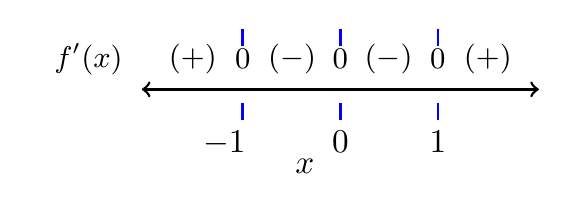
\begin{tikzpicture}[scale=1.2]
                  \begin{axis}[
                  axis y line=left,
                xlabel={$x$},
                ylabel={},
                xlabel style={anchor=west},
    	  y axis line style={draw=none},
    	  	  x axis line style={draw opacity=0},
                %grid = major,
                every major tick/.append style={ thick, blue, major tick length=5pt},
                xtick       = {-1.72, 0, 1.72},
                xticklabels = {$-1\;\;\;\;$ ,$0$,  $1$},
                ytick       = \empty,
                yticklabels={},
                                          y  axis line style=-,
                              % y axis/.append style={y axis line style=-}
                samples     = 320,
                restrict y to domain=-40:40,
                xmin = -5.5, xmax = 3.5,
                ymin = -.5, ymax = 1,
                height=1in, width=2.75in
              ]
    	\draw[thick,<->] (-3.5,0) -- (3.5,0);
    	 \node[anchor=west] at (-5.25,.5) {\small $f^{\prime}(x)$};
    	  \node at (-1.72,.5) {\small $0$};
    	  	   \node at (0,.5) {\small $0$};
    	   \node at (1.72,.5) {\small $0$};
    		\node at (-2.6,.5) {\small $(+)$};
    		\node at (-.85,.5) {\small $(-)$};
    		\node at (.85,.5) {\small $(-)$};
    		\node at (2.6,.5) {\small $(+)$};
              %
            \end{axis}
        \end{tikzpicture}
    \end{center}
    
    By the first derivative test, $f$ has a local maximum at $x=-1$, a local minimum at $x=1$, and neither a local maximum nor a local minimum at $x=0$.

    {\color{orange} Note: If the second derivative test is used for this part, it cannot be used to classify the critical number x=0. This is because $f''(0)=0$, so the second derivative test is inconclusive. Inconclusive is not neither. It means $x=0$ could be a local max, a local min, or neither, but the test can't come to a conclusion.}
\end{solution}

    \item Find the $x$-values of all absolute extrema of $f(x)$ on the interval $[0, 2]$.
\begin{solution}
    We look for values of $f(x)$ at all critical numbers in this interval, as well as the endpoints of this interval.
    
    \begin{table}[h!]
        \centering
        \color{blue}
        \begin{tabular}{c|c}
           $x$  & $f(x)$ \\\hline
            $0$ & $0-0=0$\\
            $1$ & $3-5=-2$\\
            $2$ & $3(2)^5-5(2)^3=96-40=56$\\
        \end{tabular}\
    \end{table}
    By comparing these $f(x)$ values, we conclude that on the interval $[0, 2]$, the function $f(x)$ has its absolute maximum value at $x=2$ and has its absolute minimum value at $x=1$.
    

    {\color{orange} Note: This part is asking for all absolute extrema. The closed interval method is the only suitable method because it is the only method we've learned that would give both absolute max and min. The first derivative test for absolute extrema would only give one absolute extrema, so it would not satisfy what this part is asking for.}
\end{solution}
\end{enumerate}

}

\newpage
\section{Applications of the Derivative}
\enumR{
%\item \ltrm{\target{A2}}Let $f(x)=\ln|x^2-6x|$
%(Note: it is a logarithm of the \emph{absolute value} of $x^2-6x$).
%Additionally, note that $f'(x)=\dfrac{2x-6}{x^2-6x}$ and $f''(x)=\dfrac{-2x^2+12x-36}{(x^2-6x)^2}$.
%\begin{itemize}
%\item[(a)] Find all critical numbers of $f$.
%    
%    \vfill
%    \vfill
%    
%\item[(b)] For each critical number, determine whether a local maximum, a local minimum, or neither occurs at the critical number.
%
%    \vfill
%    \vfill
%    \vfill
%
%\item[(c)] Identify the absolute extrema of $f$ on the interval $[1,4]$.
%
%    \vfill
%    \vfill
%
%\end{itemize}
%
%\newpage


\item \ltrm{\target{A3}} A movie theater has found that if they price movie tickets at \$10 each, they can sell 100 tickets. If the price of each ticket is changed to $p$, then a total number of $n(p)=120-2p$ tickets are sold. There are only 120 seats in the theater.
 
What price should the movie theater sell the tickets at to maximize the revenue?

To receive full credit, make sure to clearly state the objective function, a domain/interval for optimization, and fully justify why price you've found maximizes the revenue. 

You are required to use a method we've learned in our course, such as the first derivative test, the second derivative test, the close interval method, or the first derivative test for absolute extrema, to solve this problem. In addition, you need to make sure the method you use is suitable for the question.
\begin{solution}
Given the price $p$, the number of tickets sold at that price is $120-2p$, so the revenue function $R(p)$ is $p \cdot (120-2p)$.  (There is a reminder about the meaning/formula for revenue on the formula sheet at the back.)

The number of tickets $120-2p$ cannot be negative, so we must have $p \leq 60$.  Also the price $p$ cannot be negative.  Thus a reasonable domain is $[0,60]$.  It is okay to exclude one or both endpoints, which amounts to requiring that price or attendance be nonzero.

We need to find the \underline{absolute maximum} of the function $R(p) = p \cdot (120-2p) = 120p - 2p^2$ on the domain $[0,60]$.

Let's next find the critical values that lie in the domain, which will be relevant whichever optimization method we choose.  We have $R'(p) = 120 - 4p$, which exists everywhere and is zero when $p=30$.  So the only critical value is 30, which does lie in the domain.

The closed interval method applies, assuming endpoints of the interval were included in the domain.  We compute the revenue at endpoints and critical values in the domain: $R(0)=0$, $R(30) = 1800$, $R(60)=0$.  Thus the maximum revenue is \$1800, attained when the price is \boxed{\$30} per ticket.

OR the first derivative test for absolute extrema applies because there is one critical point in the domain, which is an interval.  One needs to compute the sign of $R'$ on either side of the critical value to get a sign chart, say $R'(10) = 80 > 0$ and $R'(50) = -80 < 0$.  This implies that the critical value of \boxed{\$30} per ticket is an absolute maximum.
\end{solution}
\newpage

\item \ltrm{\target{A3}}You are building five identical pens adjacent to each other with a
total area of $7500\ \text{m}^2$,
as shown in the following figure.
What dimensions should you use to minimize the amount of fencing?
\begin{center}
\begin{tikzpicture}[scale=1.2]
\draw (0,0) -- (5.0,0) -- (5.0,2.5) -- (0,2.5) -- (0,0);
\draw (1.0,0) -- (1.0,2.5);
\draw (2.0,0) -- (2.0,2.5);
\draw (3.0,0) -- (3.0,2.5);
\draw (4.0,0) -- (4.0,2.5);
\draw[dashed] (-.3,0) -- (-.3,2.5);
\draw (-.5,0) -- (-.1,0);
\draw (-.5,2.5) -- (-.1,2.5);
\node[font=\large] at (-.6,1.25) {$y$};
\draw[dashed] (0,2.8) -- (1,2.8);
\draw (0,2.6) -- (0,3);
\draw (1,2.6) -- (1,3);
\node[font=\large] at (.5,3.1) {$x$};
\end{tikzpicture}
\end{center}
}
\begin{solution}
{\bf Modeling phase} 
We are minimizing the amount of fencing which includes the perimeter of the rectangle as well as the fencing in the interior. I will call this amount $F$.
$$F=10x+6y$$
Since this is a function of two variables, we need to reduce it to one variable in order to minimize it. We're told that the area must be $7500$ m$^2$. Thus
\begin{align*}
A=5x\cdot y&=7500\\
y&=\frac{7500}{5x}=\frac{1500}{x}
\intertext{We use this to reduce $F$ to one variable}
F(x)&=10x+6\left(  \frac{1500}{x} \right)\\
F(x)&=10x+9000 x^{-1}
\end{align*}
The domain for this function is $0<x<\infty$.\\\\
{\bf Calculus phase} 
We find critical numbers by determining when $F^{\prime}(x)=0$ or $F^{\prime}(x)$ DNE.
\begin{align*}
F^{\prime}(x)&=10-9000 x^{-2}\\
F^{\prime}(x)&=10-\frac{9000}{x^2}
\intertext{We explore $F^{\prime}(x)=0$ }
0&=10-\frac{9000}{x^2}\\
\frac{9000}{x^2}&=10\\
\frac{9000}{10}&=x^2\\
\pm 30 =x
\end{align*}
We ignore $x=-30$ since it's not in the domain $0<x<\infty$ and thus $x=30$ is a critical number. \\\\
We now check $F^{\prime}(x)$ DNE. Since $F^{\prime}(x)=10-9000 x^{-2}$, we have a division by $0$ at $x=0$ which means $F^{\prime}(0)$ DNE.  However $x=0$ is not in the domain $0<x<\infty$ and we can ignore it. \\\\
{\bf Check for Absolute Minimum} We first check to see if $x=30$ is a {\em local minimum}.
\itemI{
\item We choose any value in the domain less than $30$, say $x=10$.  
\begin{align*}
F^{\prime}(10)&=10-\frac{9000}{10^2}=10-\frac{9000}{100}=10-900<0
\end{align*}
\item We choose any value in the domain greater than $30$, say $x=100$.  
\begin{align*}
F^{\prime}(10)&=10-\frac{9000}{100^2}=10-\frac{9000}{10000}=10-\frac{9}{10}>0
\end{align*}
}
\mpageT{.5}{.5}{
This information is captured on the sign line and we see that we have a {\em local minimum} by the First Derivative Test for Local Extrema.
}{\centering
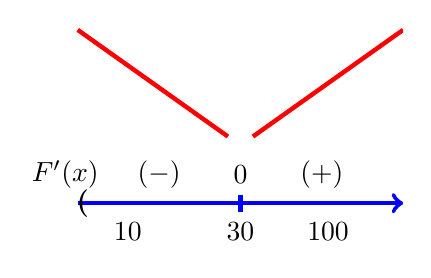
\begin{tikzpicture}
 \begin{axis}[
    	axis x line=none,
	            axis y line=none,
		x label style={anchor=west},
            xlabel={},
            xtick       = {8},
            xticklabels = {$30$},
            y label style={anchor=south},
            ylabel={},
            ytick       = {-6,-4,-2,2,4,6},
            yticklabels = {$-6$,$-4$,$-2$,$2$,$4$,$6$},
            samples     = 320,
            domain      = -2.5:2.5,
            restrict y to domain=-6.5:6.5,
            xmin = 0, xmax = 15,
            ymin = -6.5, ymax = 6.5,
            width=2.5in, height=2.5in,
            grid=none, grid style=solid
          ]
    \addplot[domain= 2:15, blue, ultra thick, mark=none, ->]{0)};
        \addplot[domain= 2:8, red, ultra thick, mark=none, -]{-4/6.5*(x-2)+6)};
         \addplot[domain= 9:15, red, ultra thick, mark=none, -]{4/6.5*(x-15)+6)};
   \draw (1.5,1) node{$\Large F^{\prime}(x)$};
   \draw (5.25,1) node{$\Large (-)$};
      \draw (11.75,1) node{$\Large (+)$};
   \draw (2.2,0) node{ \bf (};
         \draw (8.5,1) node{$0$};
   \draw[ultra thick, blue] (8.5,.3)--(8.5,-.3);
      \draw (8.5,-1) node{$30$};
       \draw (4,-1) node{$10$};
         \draw (12,-1) node{$100$};
    \end{axis}
\end{tikzpicture}
}~\\
We must now confirm that we have an {\em absolute minimum}. The domain is not a closed interval so we cannot use the closed interval method. However, we have only one critical number ($x=30$) in the domain and the sign of $F^{\prime}$ changes from negative to positive at $x=30$ Thus by the First Derivative Test for Absolute Extrema, we have an absolute minimum when $x=30$.\\\\
$\ds y=\frac{1500}{30}=50$ and the dimensions that minimize the fencing to enclose $7500$ m$^2$ are $x=30$ and $y=50$.

\end{solution}

\newpage

\section{Integrals}
\enumR{
\item \ltrm{\target{I1}} \enum{
 \item Let $r(t)$ represent the rate of energy produced by solar radiation per square meter, in kilowatts per square meter, or $kW/m^2$, on a given day, where $t$ is the number of hours since midnight.

    \begin{enumerate}
        \item[(i)] What is the unit of $\displaystyle\int_0^8 r(t)\, dt$?

\begin{solution}
        $$\frac{\text{kW}}{\text{m}^2} \times \text{hours} = \frac{\text{kW} \times \text{hours}}{\text{m}^2}$$
\end{solution}

        \item[(ii)] Explain the meaning of $\displaystyle\int_0^8 r(t)\, dt$ in this context.

\begin{solution}
The net change in the amount of energy in $\ds \frac{kW\cdot hours}{m^2}$ produced between 0 hours and 8 hours since midnight.
    
        OR The total amount of energy in $\ds \frac{kW\cdot hours}{m^2}$ produced between 0 hours and 8 hours since midnight.
\end{solution}
    \end{enumerate}

\vfill

    \item When bleeding, a human heart still pumps blood, but the amount it pumps drops over time. In particular, the function $p(t)$ represents the amount of blood pumped by the heart per minute, where $t$ represents the number of minutes after the human starts bleeding.

    \begin{enumerate}
        \item[(i)] Based on this scenario, is $\displaystyle \int_0^5 p(t)\, dt$ positive, negative, or 0? No justification required.

\begin{solution}
Positive, since the heart is still pumping blood, just at a slower rate. Thus, the amount of blood the heart pumped after 5 minutes of bleeding is positive.
\end{solution}

        \item[(ii)] Write down an expression representing the amount of blood the heart pumps from 2 minutes after the start of bleeding to 10 minutes after the start of the bleeding.

\begin{solution}
  $$\int_2^{10} p(t)dt$$
\end{solution}
    \end{enumerate}
    \vfill
    }


\newpage

\item \ltrm{\target{I2}}  Suppose the following values of definite integrals are given.

\[\int_{-1}^{2}g(x)\,dx=3\]

\[\int_{-3}^{-1}g(x)\,dx=1\]

\[\int_2^{-1}3(f(x)-g(x))\,dx=12\]

\[\int_{-3}^22(f(x)-g(x))\,dx=8\]

Find the value of the following definite integrals.

\tasksA{2}{
\task $\displaystyle\int_2^2 g(x)\, dx$\\
\begin{solution}
Since an integral over an interval of zero length is always zero, by the \textbf{``Area of a Line Segment Property"}
\\
 $\displaystyle\int_2^2 g(x)\, dx = 0$
\end{solution}

\task $\displaystyle\int_{-1}^2 f(x)\, dx$

\begin{solution}
We are given:
\[
\int_{-1}^{2} g(x)\,dx = 3,
\qquad
\int_{2}^{-1} 3(f(x)-g(x))\,dx = 12
\]
\textbf{Use ``Reverse Limits Property":}
\[
-\int_{-1}^{2} 3(f(x)-g(x))\,dx = 12
\]
\textbf{Use ``Linearity":}\\
Divide both sides by 3: (algebra)
\[
\int_{-1}^{2} (f(x)-g(x))\,dx = -4
\]
\textbf{Use ``Linearity":}
\[
\int_{-1}^{2} f(x)\,dx - \int_{-1}^{2} g(x)\,dx = -4
\]
Substitute (algebra) \(\int_{-1}^{2} g(x)\,dx = 3\):
\[
\int_{-1}^{2} f(x)\,dx - 3 = -4
\]
\[
\int_{-1}^{2} f(x)\,dx = -1
\]
So, 
\[
\displaystyle\int_{-1}^2 f(x)\, dx = -1
\]
\end{solution}

\task $\displaystyle\int_{-3}^2 f(x)\, dx$
\begin{solution}
We are given:
\[
\int_{-3}^{2} 2(f(x)-g(x))\,dx = 8
\]
\textbf{Use ``Linearity":}\\
Divide both sides by 2: (algebra)
\[
\int_{-3}^{2} (f(x)-g(x))\,dx = 4
\]
\textbf{Use ``Linearity":}
\[
\int_{-3}^{2} f(x)\,dx - \int_{-3}^{2} g(x)\,dx = 4
\]
\textbf{Use ``Break Apart Property":}\\
Substitute: (algebra)
\[
\int_{-3}^{2} g(x)\,dx
= \int_{-3}^{-1} g(x)\,dx + \int_{-1}^{2} g(x)\,dx
= 1 + 3 = 4
\]
Thus:
\[
\int_{-3}^{2} f(x)\,dx - 4 = 4
\]
\[
\int_{-3}^{2} f(x)\,dx = 8
\]
$\displaystyle\int_{-3}^2 f(x)\, dx = 8$

~\\
\textbf{Key Aspects of Problem:}
\begin{itemize}
    \item Area of a Line Segment (used once)\\
    \item Reverse Limits Property (used once)\\
    \item Break apart property (used once)\\
    \item Linearity of integration (used four times)\\
    \item Algebraic manipulations (substitution twice and division twice and addition twice)
\end{itemize}
\end{solution}
}

\newpage

\item \ltrm{\target{I3}}Assume $x>0$. Write down the indefinite integrals of the following expressions. 

Although no work is required, you are encouraged to include any work that shows your thought process. 

%constant, power, exponential, log, +C, algebraic manipulation

\begin{center}
         \begin{tabular}{l c r l c r}
            %
            $\displaystyle\int x^4+\log_2(10)\,dx$ & $=$ &\unlineb{1.5}{\ds \frac{x^5}{5}+\log_2(10)x+C}{.35} &
            %
            %$\displaystyle\int \,dx$ & $=$ & \rule[-8pt]{1.5in}{0.4pt}\\[0.3in]
            %%%%%
            %$\displaystyle\int 15\,dx$ & $=$ & \rule[-8pt]{1.5in}{0.4pt} & 
            %%%%%
            $\displaystyle\int \dfrac{3}{x^8} \,dx$ & $=$ & \unlineb{1.5}{\ds \frac{3x^{-7}}{-7}+C=-\frac{3}{7x^7}+C}{.35}  \\[.5in]
            %%%%%
            $\displaystyle\int 3^x\,dx$ & $=$ & \unlineb{1.5}{\ds \frac{3^x}{\ln(3)}+C}{.35}&
            %
            $\displaystyle\int \dfrac{1}{2x}\,dx$ & $=$ &  \unlineb{1.5}{\ds \frac{1}{2}\ln|x|+C}{.35} \\[.5in]
            %%%%%
            $\displaystyle\int 4\sqrt{x}-e^x \,dx$ & $=$ &  \unlineb{1.5}{\ds \frac{8}{3}x^{3/2}-e^x+C}{.35} & 
            %
            $\displaystyle\int \dfrac{1}{\sqrt[5]{x^3}} \,dx$ & $=$ &  \unlineb{1.5}{\ds \frac{5}{2}x^{2/5}+C}{.35} \\[0.3in]
            %%%%%
        \end{tabular}\end{center}
        
\begin{solution}
\par\noindent\hrulefill \\
\mpageT{.5}{.5}{
\al{
\int x^4+\log_2(10)\,dx&=\frac{x^5}{5}+\log_2(10)x+C\\
\intertext{($\log_2(10)$ is a constant)}
}
}{
\al{
\int \dfrac{3}{x^8} \,dx&=\int 3x^{-8}\,dx\\
&=3\frac{x^{-7}}{-7}+C\\
&=-\frac{3}{7}\cdot \frac{1}{x^7}+C
}
}
\par\noindent\hrulefill \\
\mpageT{.5}{.5}{
\al{
\int 3^x\,dx&=3^x\cdot\frac{1}{\ln(3)}+C
}
}{
\al{
\int \dfrac{1}{2x}\,dx&=\int \dfrac{1}{2}\cdot \frac{1}{x}\,dx\\
&=\frac{1}{2} \ln|x|+C
}
}
\par\noindent\hrulefill \\
\mpageT{.5}{.5}{
\al{
\int 4\sqrt{x}-e^x \,dx&=\int 4x^{1/2}-e^x \,dx\\
&=4 \cdot \frac{x^{3/2}}{3/2}-e^x +C\\
&=4 \cdot \frac{2}{3}  x^{3/2} - e^x +C\\
&=\frac{8}{3}  x^{3/2} - e^x +C\\
}
}{
\al{
\int \dfrac{1}{\sqrt[5]{x^3}} \,dx&=\int \dfrac{1}{x^{3/5}} \,dx\\
&=\int \dfrac{1}{x^{-3/5}} \,dx\\
&=\frac{x^{2/5}}{2/5}+C\\
&=\frac{5}{2}x^{2/5}+C
}
}
\par\noindent\hrulefill 
\end{solution}
\newpage

\item \ltrm{\target{I4}}For each of the following definite integrals, determine whether the Fundamental Theorem of Calculus can be applied to evaluate. 

If so, evaluate the integral using the FTC. There's no need to simplify your final answer.

If not, clearly indicate that and explain why.

\begin{enumerate}
    \item $\displaystyle\int_{-8}^{-1}\dfrac{1}{x}+e^x-\sqrt[3]{x}\, dx$

\begin{solution}
The integrand is the sum of $\dfrac{1}{x}$, $e^x$, and $-\sqrt[3]{x}=-x^{1/3}$.  On the interval $[-8,-1]$ none of these summands are discontinuous: $1/x$ is defined (zero is not in the interval) and $e^x$ and $-x^{1/3}$ are continuous for all real numbers $x$.  Hence the integrand is continuous on $[-8,-1]$ and the FTC applies.
    The definite integral is then:\\
    \[
    F(x)=\ln|x|+e^x-\frac{3}{4}x^{4/3}\bigg|_{-1}^{-8},
    \]
    since \(\dfrac{d}{dx}\ln|x|=\dfrac{1}{x},\ \dfrac{d}{dx}e^x=e^x,\ \dfrac{d}{dx}\!\left(\frac{3}{4}x^{4/3}\right)=x^{1/3}.\)
    By the FTC,
    \[
    \int_{-8}^{-1}\!\Big(\dfrac{1}{x}+e^x-\sqrt[3]{x}\Big)\,dx
    =F(-1)-F(-8).
    \]
    The evaluated result (left unsimplified) is
    \[
    \boxed{\;\textcolor{blue}{\; \ln|{-1}|+e^{-1}-\tfrac{3}{4}(-1)^{4/3}
    \;-\;\big(\ln|{-8}|+e^{-8}-\tfrac{3}{4}(-8)^{4/3}\big)\;}\;}
    \]
\end{solution}

    \item $\displaystyle\int_{-8}^1\dfrac{1}{x}+e^x-\sqrt[3]{x}\, dx$

\begin{solution}
 The integrand contains the term $\dfrac{1}{x}$, which is \emph{not} defined at $x=0$.  Because the interval $[-8,1]$ contains $0$, the integrand is not continuous on the entire closed interval $[-8,1]$.  The Fundamental Theorem of Calculus requires the integrand to be continuous on $[a,b]$ in order to apply directly; therefore the FTC \emph{cannot} be applied as stated.\\
    \boxed{\;\textcolor{blue}{\text{FTC cannot be applied because } \dfrac{1}{x}\text{ is undefined at }x=0 \text{ and } 0 \in [-8,1].}\;}
    

\end{solution}
\end{enumerate}

}
\blue{
    \textbf{Key Aspects of Problem:}
\begin{itemize}
    \item FTC applies to first integral\\
    \item If students conclude that first integral does not satisfy FTC, a domain reason should be given. (Note: the use absolute value in the antiderivative for $\dfrac{1}{x}$ is not being tested on, hence it is not required. So solutions of the form $\ln(-8) - \ln(-1)$ should be counted as valid.)\\
    \item Correct usage of the FTC as the difference in boundary values.\\
    \item Second part does not satisfy FTC\\
    \item Correct reasoning as to why second part does not satisfy FTC. (If students conclude that the second problem does satisfy FTC, a correct implementation should be given with the assumption that it does satisfy the FTC)
\end{itemize}
}
\newpage




\section{Discrete and Continuous Probability Distributions} 
\itemI{
\item A {\em discrete probability distribution} is discrete because the set of outcomes is discrete: In the case of the sum of the roll of 2 dice die we had outcomes $\{2,3,4,\dots,12\}$.  In general, our set of outcomes will be  $\{x_1, x_2, x_3,\dots x_n\}$ where $n$ could also head towards infinity.
\item A {\em continuous probability distribution} is continuous because the set of outcomes of an experiment is continuous.  (e.g. measuring the height of a person, determining the wait time at the DMV, weighing a Roots Bowl, etc).
}
\enumR{
\item  \ltrm{\target{P1}}$X$ is the random variable that describes rolling two $6$-sided dice.The table below contains all possible rolls of two dice and the corresponding sums. You will find it helpful to answer the following questions.
\begin{center}
\renewcommand{\arraystretch}{1.4}
\begin{tabularx}{4.in}{|K{.4}{lightgray}|C{\sz}|C{\sz}|C{\sz}|C{\sz}|C{\sz}|C{\sz}|}\cline{1-7}
\rowcolor{lightgray}
 \diagbox{\hs{-.1}\text{\footnotesize  \bf Die 1}}{\hs{-.1}\text{\footnotesize \bf Die 2}}&1&2&3&4&5&6 \\ \cline{1-7}
 1&2&3&4&5&6&7 \\ \cline{1-7}
  2&3&4&5&6&7&8 \\ \cline{1-7}
3&4&5&6&7&8&9 \\ \cline{1-7}
4&5&6&7&8&9&10 \\ \cline{1-7}
5&6&7&8&9&10&11 \\ \cline{1-7}
6&7&8&9&10&11&12 \\ \cline{1-7}
\end{tabularx}
\end{center}
\tasksA{2}{
\task What is the support $S_X$? That is, what is the set of all possible outcomes from adding together the face values of two dice after one roll of the $2$ dice?  
\sol{ 
The set of outcomes:\\ $S_X=\{2,3,4,5,6,7,8,9,10,11,12\}$
}
\task How many different ways can two dice be rolled?   Note that  first rolling a $2$ and then a $1$ is distinct from first rolling a $1$ and then a $2$.  
\sol{
\item There are 6 outcomes for first die and 6 for the second die, for a total of $6\times 6=36$
}

 \vspace{.5in}
\task* What is $p(4)=P(X=4)$?  It might be helpful to think about how many total combinations of dice rolls will yield a sum of $4$ relative to the total possible number of combinations that lead to our set of outcomes.
\sol{ From the table we see there are $3$ ways to roll a $4$: $3+1$, $1+3$, and $2+2$. Thus the probability is $\dfrac{3}{36}=\dfrac{1}{12}$}\
\vs{.25}\\
\task What is $P(X\leq 4)$?
\sol{ \alnonum{ P(X\leq 4)&=P(X=2)+P(X=3)+P(X=4)\\
&=\frac{1}{36}+\frac{2}{36}+\frac{3}{36}\\
&=\frac{6}{36}=\frac{1}{6}}
}
\task What is $P(X\leq 4)+P(X\geq 5)$?
\sol{ This is the sum of all possible\\outcomes which must be $1$.}
}
%%%%%%%%%%
\newpage
%%%%%%%%%%
\item  \ltrm{\target{P1}}$X$ is the random variable that describes rolling two $4$-sided dice.The table below contains all possible rolls of two dice and the {\em difference} between the second die and the first die.  You will find it helpful to answer the following questions.
\begin{center}
\renewcommand{\arraystretch}{1.4}
\begin{tabularx}{2.8in}{|K{.5}{lightgray}|C{\sz}|C{\sz}|C{\sz}|C{\sz}|} \cline{1-5}
\rowcolor{lightgray}
 \diagbox{\hs{-.1}\text{\footnotesize  \bf Die 1}}{\hs{-.1}\text{\footnotesize \bf Die 2}}&1&2&3&4 \\ \cline{1-5}
  1&0&1&2&3 \\ \cline{1-5}
    2&-1&0&1&2 \\ \cline{1-5}
3&-2&-1&0&1 \\ \cline{1-5}
4&-3&-2&-1&0 \\ \cline{1-5}
\end{tabularx}
\end{center}
\tasksA{2}{
\task What is the support $S_X$? That is, what is the set of all possible outcomes from subtracting together the face values of two dice after one roll of the $2$ dice?  
\sol{
$S_{X}=\{-3, -2, -1, 0, 1, 2, 3 \}$
}
\task How many different ways can the two dice be rolled?   Note that  first rolling a $2$ and then a $1$ is distinct from first rolling a $1$ and then a $2$.  
There are 4 outcomes for first die and 4 for the second die, for a total of $4\times 4=16$
 \vspace{.5in}
\task What is $p(0)=P(X=0)$?  It might be helpful to think about how many total combinations of dice rolls will yield a difference of $0$ relative to the total possible number of combinations that lead to our set of outcomes.
\sol{
There are $4$ different ways to roll a difference of $0$ so $\ds P(X=0)=\frac{4}{16}=0.25$
}
\task Create a histogram containing probabilities for all elements of the support $S_{X}$. Note that you will want to label the horizontal axis with each element of the support.\\
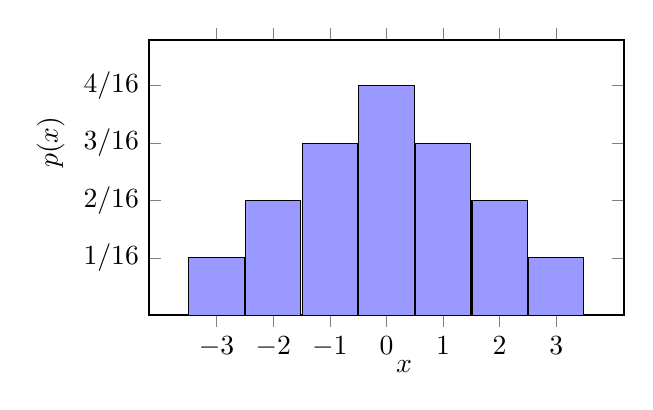
\begin{tikzpicture}
    \begin{axis}[
        ybar, % Specifies vertical bars
        bar shift=0,
        ymin=0, % Ensures bars start from zero
        xtick={1,2,3,4,5,6,7}, % Places x-axis ticks at data points
	%xticklabels={,,,,,,}, % Custom x-axis labels
	xticklabels={$-3$,$-2$,$-1$,$0$,$1$,$2$,$3$},
	ytick       = {1/16, 2/16, 3/16, 4/16},
            yticklabels =  {$1/16$,$2/16$,$3/16$, $4/16$},
        enlarge x limits={0.2}, % Adjusts spacing between bars and axis limits
            y label style={anchor=south west},
            ylabel={$p(x)$},
                        xlabel = {$x$},
		x label style={anchor=west},
		 ymin = 0, ymax = .3,
        bar width=20pt, % Adjusts the width of the bars
                    width = 3in, height=2in,
                    axis line style={thick, ->},
                    %enlarge x limits={1.2}
       % legend style={at={(0.5,-0.15)},anchor=north,legend columns=-1} % Legend positioning
    ]
% \addplot[fill=blue!40] coordinates {(1,0)  (2,0)  (3,0) (4,0) (5,0) (6,0) (7,0) };
 \addplot[fill=blue!40] coordinates {(1,0.0625)  (2,0.125)  (3,0.1875) (4,0.25) (5,0.1875) (6,0.125) (7,0.0625) };
    \end{axis}
\end{tikzpicture}

\vs{.25}
\task Find the average difference for one roll of $2$ dice. That is, what's $E[X]$?
\sol{
\al{
&\mu=E[X]=\sum_{k=-3}^{3}k\cdot p(k)\\
&=-3\cdot\frac{1}{16}+(-2)\cdot\frac{2}{16}+(-1)\cdot\frac{3}{16}+ 0\cdot\frac{4}{16}\\
&\qquad \qquad+1\cdot\frac{3}{16}+2\cdot\frac{2}{16}3\cdot\frac{1}{16}\\
&=\frac{-3}{16}+\frac{-4}{16}+\frac{-3}{16}++\frac{3}{16}+\frac{4}{16}+\frac{3}{16}\\
&=0
}
}
\task What is $Var(X)$? There's no need to simplify after setting this up.
\sol{
We have two approaches to finding the variance. Both are equivalent to ``Variance is the average of differences  from the mean squared``''\\
{\bf Approach $\#1$}\\
\al{
&Var(X)=\sum_{k=-3}^3 (k-\mu)^{2}p(k)=(-3-0)^2\frac{1}{16}+(-2-0)^2\frac{2}{16}\\
&\qquad +(-1-0)^2\frac{3}{16}+(-1-0)^2\frac{3}{16}+(-2-0)^2\frac{2}{16}\\
&\qquad +(0-0)^2\frac{4}{16}+(1-0)^2\frac{3}{16}+(2-0)^2\frac{2}{16}+(3-0)^2\frac{1}{16}
\intertext{On an exam, it's ok to stop with previous line}
&\qquad=\frac{9}{16}+\frac{8}{16}+\frac{3}{16}+0+\frac{3}{16}+\frac{8}{16}+\frac{9}{16}\\
&=\frac{40}{16}=2.25
}
So $Var(X)=2.25$\\
{\bf Approach $\#2$}\\
\al{
&Var(X)=\left( \sum_{k=-3}^3 k^2\cdot p(k)\right)-\mu^2\\
&=\Bigg( (-3)^2\frac{1}{16}+(-2)^2\frac{2}{16}+(-1)^2\frac{3}{16}+(0)^2\frac{4}{16} \\
&\qquad+(1)^2\frac{2}{16}+(2)^2\frac{2}{16}+(3)^2\frac{1}{16} \Bigg)-0^2\\
&=\Bigg( \frac{9}{16}+\frac{8}{16}+\frac{3}{16}+0+\frac{3}{16}+\frac{8}{16}+\frac{9}{16}\Bigg) -0^2\\
&=\frac{40}{16}=2.25
}
}
}

}
%%%%%%%%%%%
\newpage
%%%%%%%%%%%


%%%%%%%%%%%%%%%%%%%  Bus stop problem  %%%%%%%%%%%%%%%
\enumR{
\item  \ltrm{\target{P2}}We're going to determine the probability of catching the bus at the stop on McIntyre between Monroe Hall and the amphitheater.  We assume that a bus comes every $10$ minutes and $T$ is a random variable that represents the wait time to catch the bus.  One probability density function (pdf) for this scenario is shown below. Note that   there's a low probability that a person will have to wait $0$ to $1$ minutes to catch the bus. There's also a low probability that a student will have to wait between $9$ and $10$ minutes to catch the bus.  But, there's a much higher probability that a person will catch the bus in between $4$ and $6$ minutes.  The pdf and graph of the pdf are below.\\
\mpageT{.5}{.5}{
\vs{.3}
\scalebox{1.2}{
$ \ds p(t)=\left\{
\begin{array}{ll}
\frac{1}{25}t&\qquad 0\leq t \leq 5\\
-\frac{1}{25}t+\frac{2}{5}&\qquad 5<t\leq 10
\end{array}
\right.
$
}
}{\centering
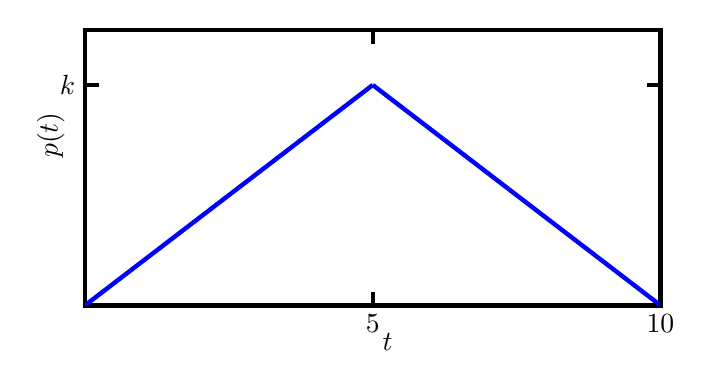
\begin{tikzpicture}
\begin{axis}[
	x label style={anchor=west},
xlabel={$t$},
xtick       = {5,10},
%xticklabels = {$10$,$20$,$30$},
xticklabel style={anchor=north},
y label style={anchor=west},
ylabel={$p(t)$},
%ytick=\empty,
%ytick       = {1/30},
ytick={0.2},
yticklabels = {$k$},
samples     = 320,
%domain      = -2.5:2.5,
%restrict y to domain=-6.5:6.5,
xmin =0, xmax = 10,
ymin = 0, ymax = .25,
axis line style = { ultra thick, -},
every major tick/.append style={ultra thick, black, major tick length=5pt},
width=3.5in, height=2in
%  grid=both, grid style=solid
]
    \addplot[domain=0:5, blue, ultra thick, mark=none]{1/25*x};
     \addplot[domain=5:10, blue, ultra thick, mark=none]{-1/25*x+2/5};
\end{axis}
\end{tikzpicture}
}
\tasksA{2}{
\task What's the probability that a person will wait $2.5$ minutes or less? That is, find $P(T\leq 2.5)$.
\sol{
\al{
P(T\leq 2.5)&\int_0^{2.5}p(t)\;dt\\
&=\int_0^{2.5}\frac{1}{25}\cdot t\;dt\\
&=\frac{1}{25}\cdot \frac{t^2}{2}\Bigg|_0^{2.5} \\
&=\frac{(2.5)^2}{50}-\frac{0^2}{50}\\
&=\frac{6.25}{50}\\
&=12.5\%
}
}
\task  What's the probability that a person will wait exactly $5$ minutes? That is, find $P(T= 5)$.
\sol{
$\ds \int_5^5p(t)\;dt=0$\\\\
It turns out that for every Continuous PDF $p(t)$, $\ds P(T=a)=\int_a^af(t)\;dt=0$. This is distinct from Discrete PDFs where $P(X=a)$ is almost always greater than 0.
}
}
\mpageT{.45}{.45}[\hs{.3}]{
\tasksAR{1}{
\task Let's now assume that it's equally likely that it will take $0-1$ minutes to catch the bus as $1-2$ minutes, as $2-3$ minutes, etc. That is, the wait time is uniformly distributed.  A probability density function that could represent this situation is below. Find a value of $k$ that will guarantee that this is a continuous probability distribution over $0\leq t\leq 10$.
}
\sol{
 It must be the case that 
\alnonum{\int_0^{10}p(t)\;dt&=1\\
\int_0^{10}k\;dt&=1\\
k\cdot t\Big|_0^{10}&=1\\
10k&=1\\
k&=\frac{1}{10}
}
}
}{\centering
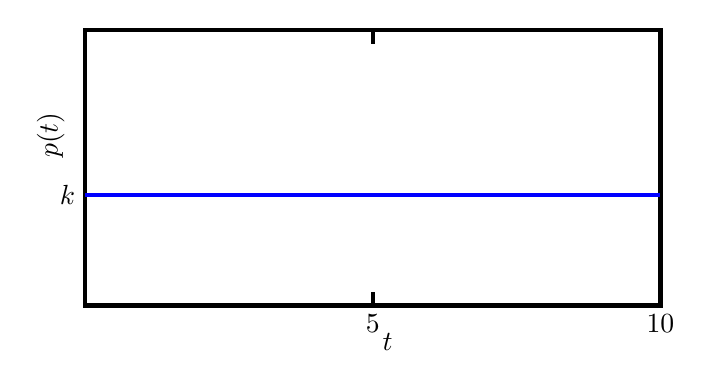
\begin{tikzpicture}
\begin{axis}[
	x label style={anchor=west},
xlabel={$t$},
xtick       = {5,10},
%xticklabels = {$10$,$20$,$30$},
xticklabel style={anchor=north},
y label style={anchor=west},
ylabel={$p(t)$},
%ytick=\empty,
%ytick       = {1/30},
ytick={0.1},
yticklabels = {$k$},
samples     = 320,
%domain      = -2.5:2.5,
%restrict y to domain=-6.5:6.5,
xmin =0, xmax = 10,
ymin = 0, ymax = .25,
axis line style = { ultra thick, -},
every major tick/.append style={ultra thick, black, major tick length=5pt},
width=3.5in, height=2in
%  grid=both, grid style=solid
]
    \addplot[domain=0:10, blue, ultra thick, mark=none]{0.1};
\end{axis}
\end{tikzpicture}
}

\newpage
\item The expected value (or mean) of a continuous random variable $X$ is $\ds \mu=E[X]=\int_1^5k\;dx$ where $k$ is an unknown constant that we will find later. 
\tasksA{2}{
    \task  What is the probability density function $p(x)$? Your answer will involve $k$.
\begin{solution}
    In general, we know that 
    \begin{align*}
mu=E[X]&=\int_1^5x\cdot p(x)\;dx
\intertext{We are also given}
\mu=E[X]&=\int_1^5k\;dx\\
    \text{Since } \int_1^5x\cdot p(x)\;dx& = \int_1^5k\;dx\intertext{ it must be the case that}
    x\cdot p(x)&=k\\
        \intertext{ and thus}  p(x)&=\frac{k}{x}
\end{align*}  

    
\end{solution}

    \task Find the value of $k$ to ensure that $p(x)$ is a pdf.  {em Hint}:  You will want to use the fact that $\ln(1)=0$
    \sol{
    The total of all probabilities must be $1$. Therefore 
    \al{
    \int_1^5p(x)\;dx&=1\\
        \int_1^5 \frac{k}{x}\;dx&=1\\
        k \int_1^5 \frac{1}{x}\;dx&=1\\
        k\cdot \ln|x| \Bigg|_1^5&=1\\
        k\ln|5|-k\ln|1|&=1\\
        k\ln|5|-0&=1 \qquad \text{ (since $\ln(1)=0$)}\\
        k&=\frac{1}{\ln(5)}
    }
    Thus $\ds p(x)=\frac{k}{x}=\frac{1/ \ln(5)}{x}=\frac{1}{\ln(5)x}$
    }
        
    \task Find the cumulative distribution function (CDF) $F(x)$.
    \begin{solution}
We're looking for the function $$F(x)=P(X\leq x)$$ for any value of $x$ in the support of $X$.
\begin{align*}
F(x)=P(X\leq x)&=\int_1^x p(w)\;dw\\
&=\int_1^x \frac{1}{\ln(5)x}\;dw\\
&=\frac{\ln|w|}{\ln(5)}\Bigg|_1^x\\
&=\frac{\ln|x|}{\ln(5)}-\frac{\ln|1|}{\ln(5)}\\
&=\frac{\ln|x|}{\ln(5)}-0 \text{ (since $\ln|1|=0$)}\\
F(x)&=\frac{\ln|x|}{\ln(5)}
\end{align*}
\end{solution}
    \task Use $F(x)$ to find $P(X \leq 4)$.
    \begin{solution}
\begin{align*}
P(X \leq 4)&=F(4)\\
&=\frac{\ln|4|}{\ln(5)}\\
&\approx 0.861 \text{ (via calculator)}
\end{align*}
\end{solution}
    \task Find $\ds \mu=E[X]$ 
    \sol{
    \al{
    \mu=E[X]&=\int_1^5x\cdot p(x)\;dx\\
    &=\int_1^5x\cdot \frac{1}{\ln(5)x}\;dx\\
    &=\int_1^5  \frac{1}{\ln(5)}\;dx\\
    &=\frac{1}{\ln(5)}\cdot x \Bigg|_1^5\\
    &=\frac{5}{\ln(5)}-\frac{1}{\ln(5)}\\
  \mu  &=\frac{4}{\ln(5)}\\
  \mu&\approx 2.49\text{ (via calculator)}
    }
    }
    \task Find $Var(X)$
    \begin{solution}
We have $2$ options: 
\begin{align*}
\text{Option $1$: } Var(X)&=\int_a^b (x-\mu)^2p(x)\;dx\\
\text{Option $2$: } Var(X)&=\left(\int_a^b x^2p(x)\;dx\right)-\mu^2
\intertext{I will use the second version since the algebra is typically easier to deal with.}
Var(X)&=\left(\int_1^5 x^2\cdot \frac{1}{\ln(5)x}\;dx\right)-\left( \frac{4}{\ln(5)}\right)^2\\
&=\left(\int_1^5 x\cdot \frac{1}{\ln(5)}\;dx\right)-\left( \frac{4}{\ln(5)}\right)^2\\
&=\left(\frac{x^2}{2}\cdot \frac{1}{\ln(5)}\Bigg|_1^5\right)-\left( \frac{4}{\ln(5)}\right)^2\\
&=\left(\frac{5^2}{2}\cdot \frac{1}{\ln(5)}- \frac{1^2}{2}\cdot \frac{1}{\ln(5)}\right)-\left( \frac{4}{\ln(5)}\right)^2\\
&=\left(\frac{25}{2}\cdot \frac{1}{\ln(5)}- \frac{1}{2}\cdot \frac{1}{\ln(5)}\right)-\left( \frac{4}{\ln(5)}\right)^2\\
&=\frac{24}{2}\cdot \frac{1}{\ln(5)}-\left( \frac{4}{\ln(5)}\right)^2\\
Var(X)&=\frac{12}{\ln(5)}-\left( \frac{4}{\ln(5)}\right)^2\\
Var(X)&\approx 1.28 \text{ (via calculator)}
\end{align*}
\end{solution}
    }

}

%\newpage
%%%%%%%%%%%%%%%%%%%  Extra Problem  %%%%%%%%%%%%%%%
%\item Gaming problem \#$1$  
%\itemI{
%\item {\bf Experiment} Bet $\$40$ each time coin is flipped. Heads means bettor receives original bet back and an additional $\$40$. Tails means bettor loses original bet.
%\item {\bf Discrete Random Variable}  $X$ is the random variable describing how much money you have after (randomly) flipping a coin only once. 
%\item Start with $\$40$
%}
%\tasksA{2}{
%	\task What is sample space of Experiment 1 of  flipping coin only once?
%	\task What is the support $S_X$?\vs{1}
%
%	\task* Create a histogram that represents the probability of arriving at each of the outcomes in $S_X$. 
%	\graphicsL{axesHistogram}{2.}	
%	}
%	\vs{.5}
%\item Gaming problem \#$2$  
%\itemI{
%\item {\bf Experiment} Bet $\$40$ each time coin is flipped. Heads means bettor receives original bet back and an additional $\$40$. Tails means bettor loses original bet.
%\item {\bf Discrete Random Variable}  $X$ is the random variable describing how much money you have after (randomly) flipping a coin twice. 
%\item Start with $\$80$
%}
%\tasksA{2}{
%	\task What is sample space of Experiment 2 of  flipping coin twice?
%	\task What is the support $S_X$?\vs{1}
%
%	\task* Create a histogram that represents the probability of arriving at each of the outcomes in $S_X$. 
%	\graphicsL{axesHistogram}{2.}	
%	}
%	\newpage
%	\item {\bf Challenge Question} (only if time): Start with \$120 and bet  $\$40$ each time coin is flipped. Heads means bettor receives original bet back and an additional $\$40$.  Player stops either when they run out of money or when they reach $\$200$. Which is more likely-- they run out of funds first or reach $\$200$ first?  An informal argument using  probabilities is ok here.  For a bigger challenge, find the probability that they run out of funds first. \vs{4}
%	
%}

\end{document}